\documentclass[12pt,a4paper]{article}
\usepackage[margin=1in]{geometry}
\usepackage{graphicx}
\usepackage{hyperref}
\usepackage{enumitem}
\usepackage{booktabs}
\usepackage{xcolor}
\usepackage{amssymb}
\usepackage{fancyhdr}
\usepackage{titlesec}
\usepackage{listings}
\usepackage{caption}
\usepackage{float}

\definecolor{primary}{RGB}{30,64,175}
\definecolor{codebg}{RGB}{245,245,250}
\definecolor{codetext}{RGB}{40,40,40}

\lstset{
  backgroundcolor=\color{codebg},
  basicstyle=\ttfamily\small\color{codetext},
  breaklines=true,
  frame=single,
  rulecolor=\color{gray!30},
  xleftmargin=0.5cm,
  framexleftmargin=0.5cm,
  numbers=none,
  showstringspaces=false,
}

\hypersetup{
  colorlinks=true,
  linkcolor=primary,
  urlcolor=primary,
  citecolor=primary,
}

\pagestyle{fancy}
\fancyhf{}
\fancyhead[L]{\small CSE 345/545 --- Foundations to Computer Security}
\fancyhead[R]{\small Milestone 2 Report}
\fancyfoot[C]{\thepage}
\renewcommand{\headrulewidth}{0.4pt}

\titleformat{\section}{\large\bfseries\color{primary}}{}{0em}{}
\titleformat{\subsection}{\normalsize\bfseries\color{primary!80!black}}{}{0em}{}

\begin{document}

% ============= TITLE PAGE =============
\begin{titlepage}
\centering
\vspace*{2cm}
{\Huge\bfseries\color{primary} VajraKavach\par}
\vspace{0.5cm}
{\Large Secure Job Search \& Professional Networking Platform\par}
\vspace{2cm}
{\LARGE\bfseries Project Milestone 2 Report\par}
\vspace{0.3cm}
{\large CSE 345/545: Foundations to Computer Security\par}
\vspace{2cm}

\begin{tabular}{ll}
\toprule
\textbf{Team Members} & \textbf{Roll Number} \\
\midrule
Yash Kumar Vaibhav & MT25091 \\
Aayush Gupta & MT25008 \\
Ayush Jain & MT25066 \\
Ayush Kumar & 2020290 \\
\bottomrule
\end{tabular}

\vspace{2cm}
{\large Indraprastha Institute of Information Technology, Delhi\par}
\vspace{0.3cm}
{\large February 27, 2026\par}
\vfill
\end{titlepage}

% ============= CONTENT =============
\tableofcontents
\newpage

% ============================================================
\section{Secure User Registration and Login}
% ============================================================

\subsection{Overview}
VajraKavach implements a multi-layered authentication system with industry-standard security practices. The registration and login flow ensures no plaintext passwords are ever stored or transmitted unnecessarily.

\subsection{Registration Flow}
\begin{enumerate}
  \item User submits email, full name, password, and role (job\_seeker / recruiter).
  \item \textbf{Server-side validation:} Email format, password strength (minimum 8 chars, must contain uppercase, lowercase, digit, and special character).
  \item \textbf{Password hashing:} Password is hashed using \textbf{Argon2id} (memory-hard, resistant to GPU/ASIC attacks) via the \texttt{passlib} library.
  \item \textbf{PKI key pair generation:} An RSA-2048 key pair is generated for the user. The public key is stored in plaintext; the private key is encrypted with \textbf{Fernet (AES-128-CBC)} before storage.
  \item \textbf{TOTP secret generation:} A unique TOTP secret is generated using \texttt{pyotp} and stored for subsequent two-factor authentication.
  \item User record is created in PostgreSQL with all security fields populated.
\end{enumerate}

\subsection{Login Flow}
\begin{enumerate}
  \item User submits email and password.
  \item Server retrieves the user record and verifies the password against the Argon2id hash.
  \item On success, a \textbf{JWT access token} (HS256, 30-minute expiry) is issued.
  \item The JWT payload includes the user ID, role, and \textbf{client IP address} for session binding.
  \item A refresh token (7-day expiry) is also issued for seamless session renewal.
  \item The \texttt{get\_current\_user} dependency validates the JWT on every protected request and verifies the IP matches the token's bound IP (preventing session hijacking).
\end{enumerate}

\subsection{Security Features}
\begin{table}[H]
\centering
\begin{tabular}{ll}
\toprule
\textbf{Feature} & \textbf{Implementation} \\
\midrule
Password Hashing & Argon2id (memory: 65536 KB, iterations: 3, parallelism: 4) \\
JWT Tokens & HS256, 30-min access / 7-day refresh \\
IP Binding & Client IP embedded in JWT, validated on each request \\
Rate Limiting & Account suspension after repeated failures \\
Input Validation & Pydantic schemas with strict email/password rules \\
\bottomrule
\end{tabular}
\caption{Authentication Security Summary}
\end{table}

\subsection{Screenshots}

\begin{figure}[H]
\centering
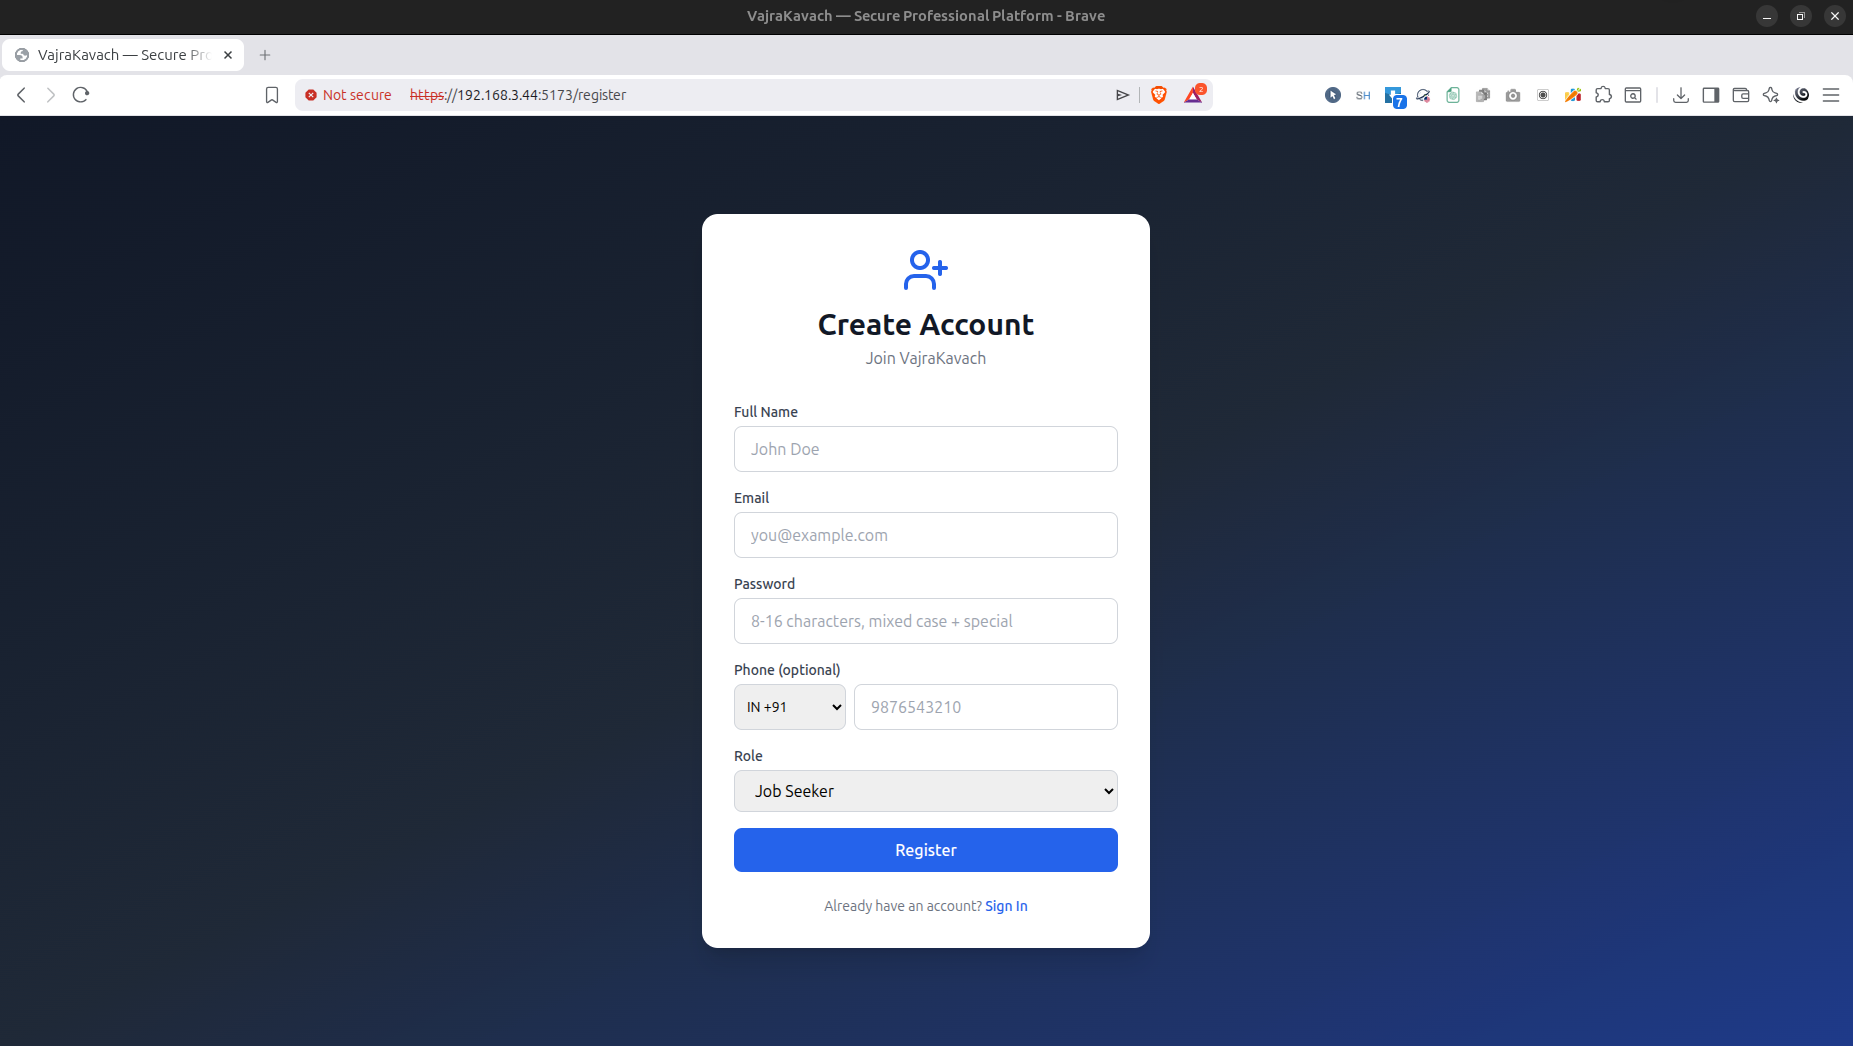
\includegraphics[width=0.85\textwidth]{screenshots/m2_registration.png}
\caption{User registration page with email, name, password, and role selection}
\end{figure}

\begin{figure}[H]
\centering
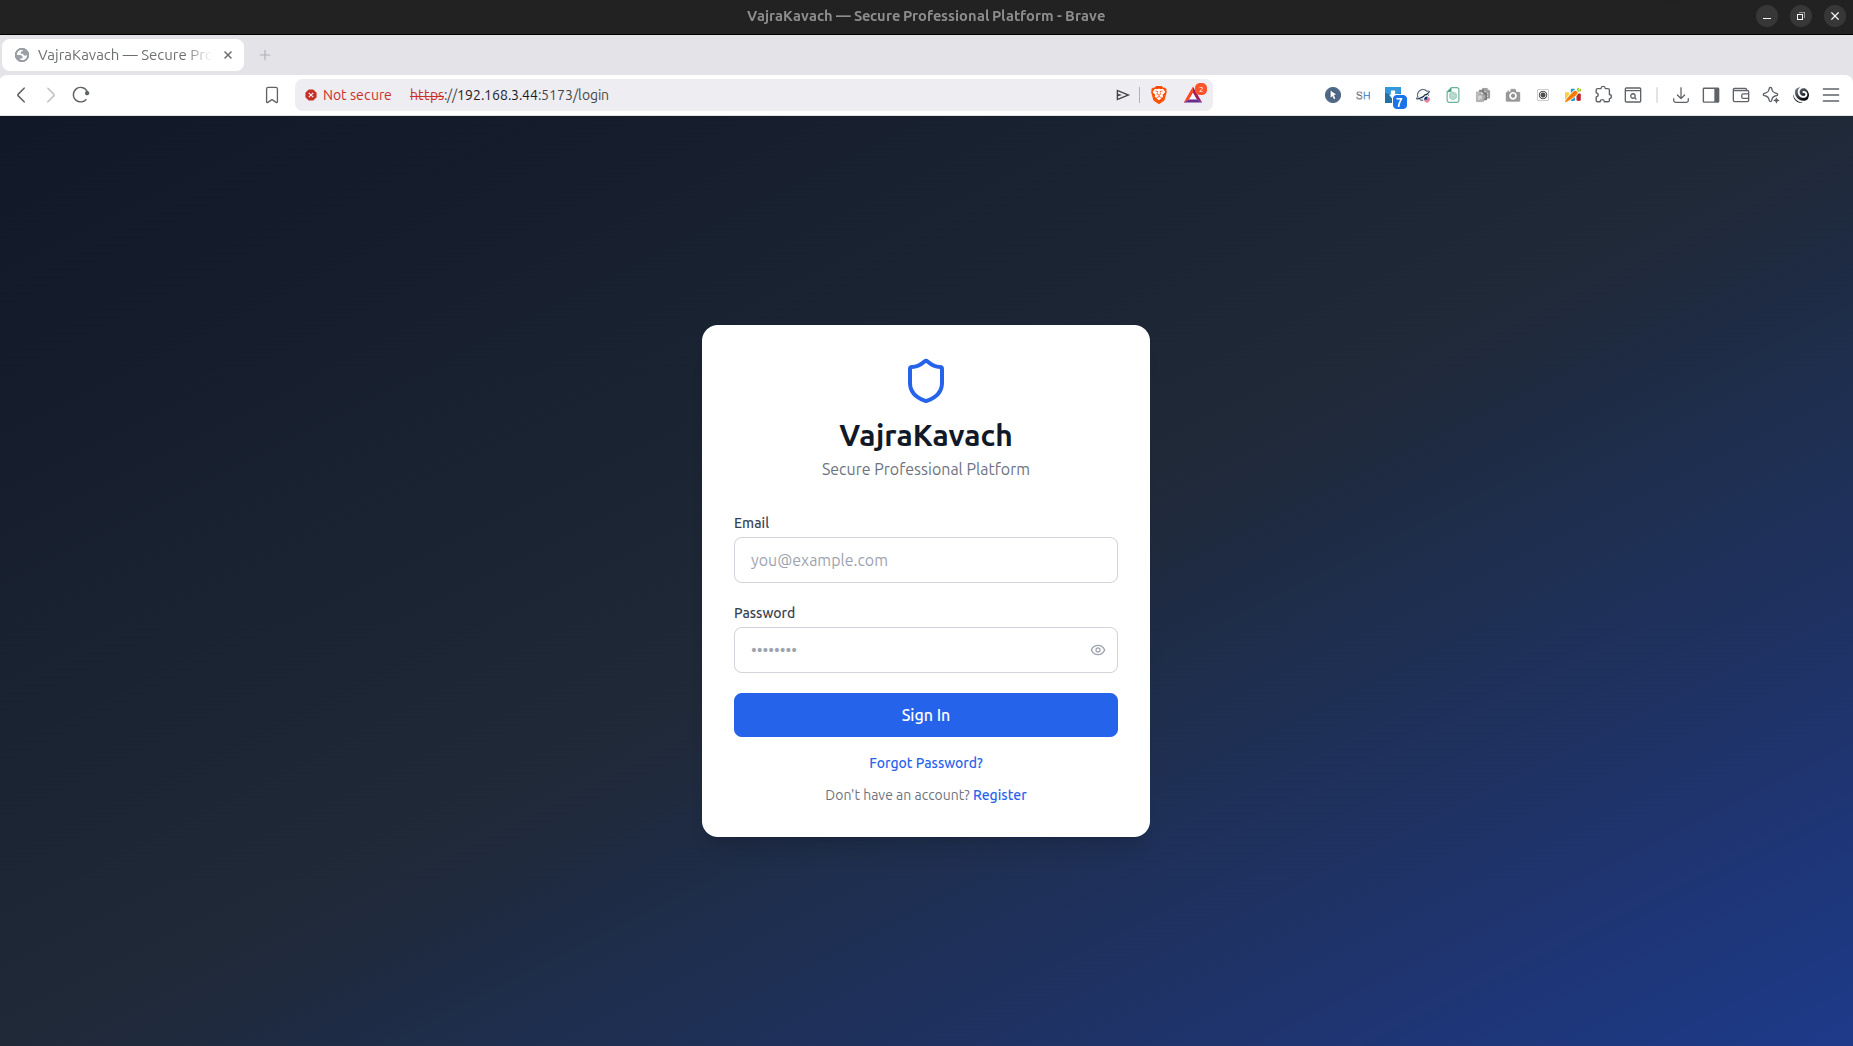
\includegraphics[width=0.85\textwidth]{screenshots/m2_login.png}
\caption{Login page with email and password fields}
\end{figure}

\newpage

% ============================================================
\section{TOTP Verification}
% ============================================================

\subsection{Overview}
Time-based One-Time Password (TOTP) is implemented as a \textbf{mandatory second factor} after login. Users must set up TOTP during their first login and verify it on every subsequent login.

\subsection{TOTP Setup Flow}
\begin{enumerate}
  \item After first login, the user is presented with a QR code containing their TOTP secret.
  \item The QR code is generated server-side using the \texttt{qrcode} library and follows the \texttt{otpauth://} URI standard.
  \item User scans the QR code with an authenticator app (Google Authenticator, Authy, etc.).
  \item User enters a 6-digit TOTP code to verify setup.
  \item On successful verification, the TOTP is marked as verified in the database.
\end{enumerate}

\subsection{TOTP Verification on Login}
\begin{enumerate}
  \item After email/password validation, the server checks if TOTP is verified.
  \item User is prompted to enter the current 6-digit TOTP code.
  \item Server validates the code using \texttt{pyotp.TOTP.verify()} with a ±1 window tolerance.
  \item On success, a new JWT token is issued with full authentication status.
\end{enumerate}

\subsection{TOTP for High-Risk Actions}
TOTP verification is additionally required for:
\begin{itemize}
  \item \textbf{Resume download:} Recruiters must enter TOTP before downloading any candidate's resume.
  \item \textbf{Resume deletion:} Users must verify TOTP before deleting their own resume.
  \item \textbf{Password change:} Current password + TOTP required.
\end{itemize}

\subsection{Screenshots}

\begin{figure}[H]
\centering
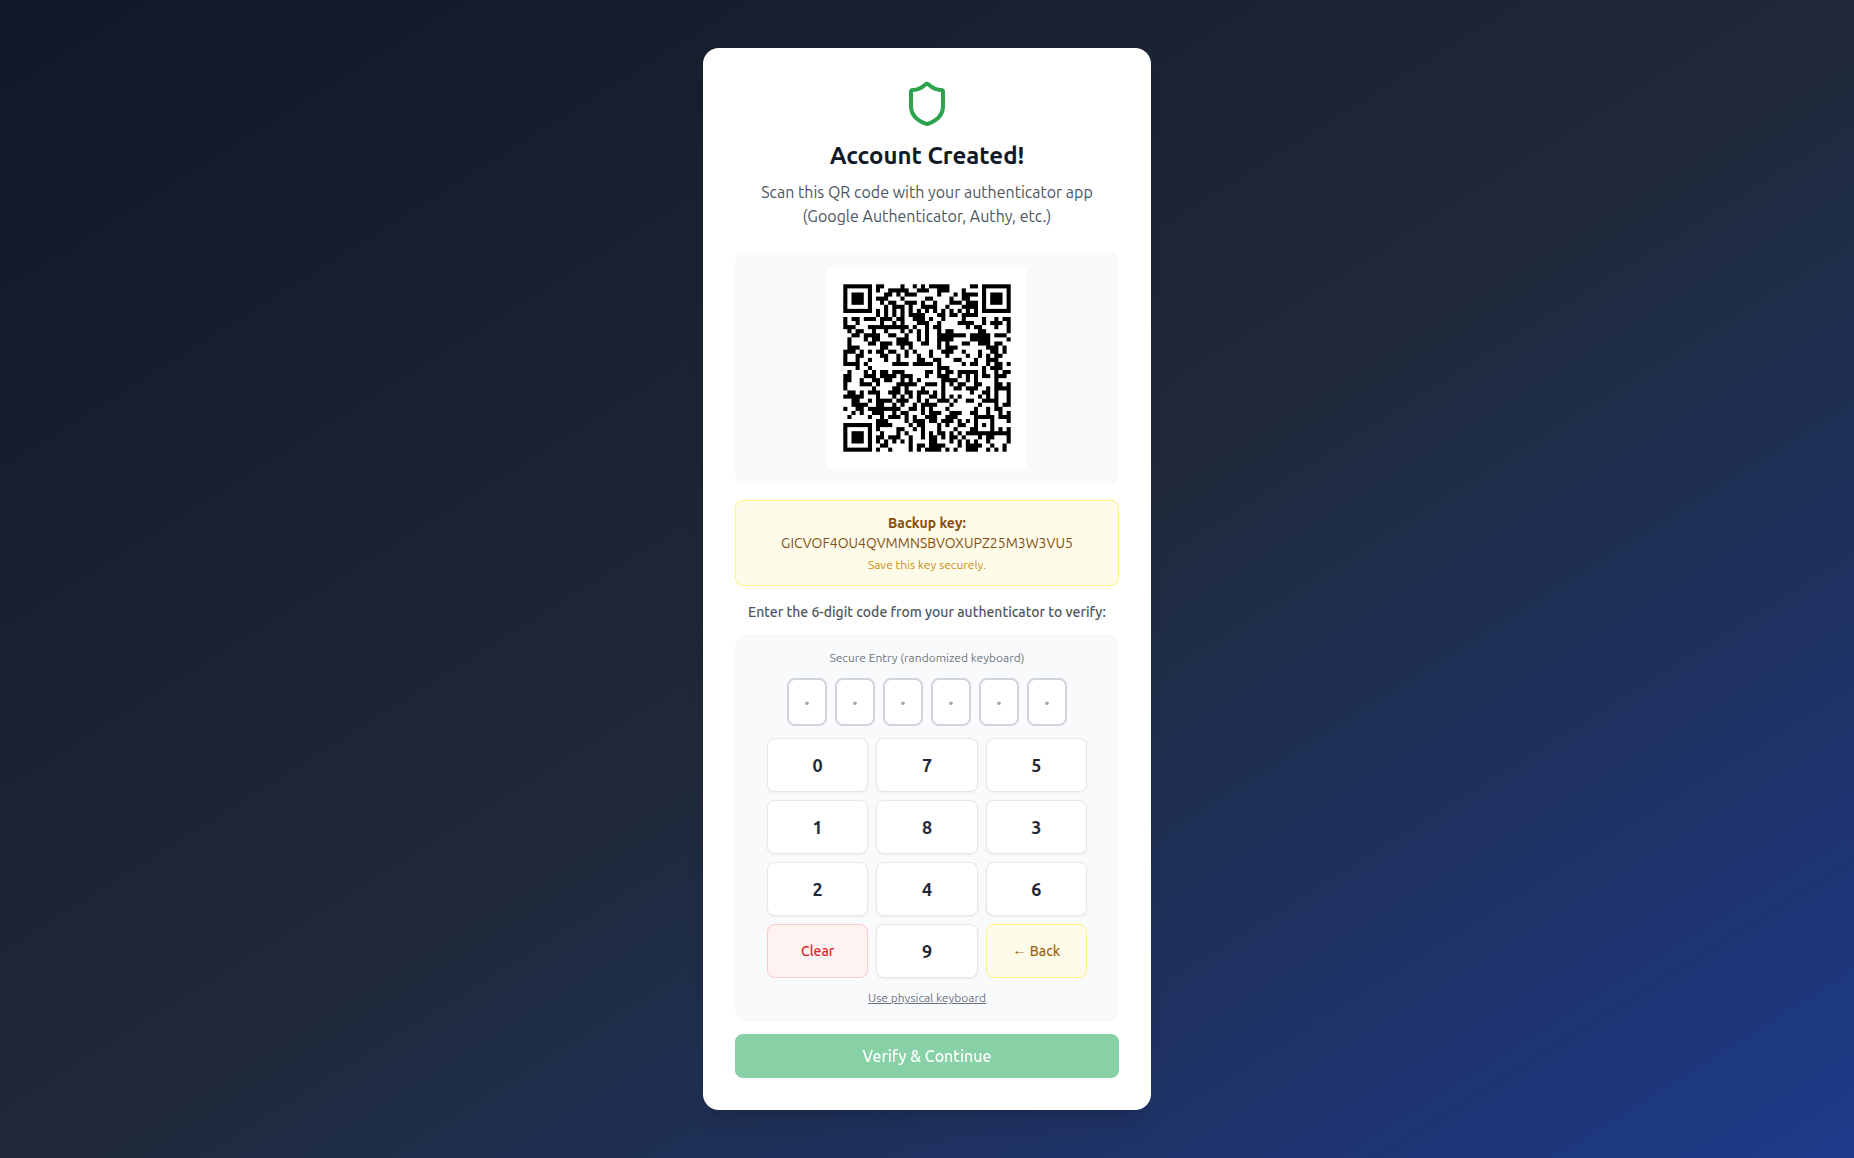
\includegraphics[width=0.7\textwidth]{screenshots/m2_totp_setup.png}
\caption{TOTP setup screen showing QR code for authenticator app}
\end{figure}

\begin{figure}[H]
\centering
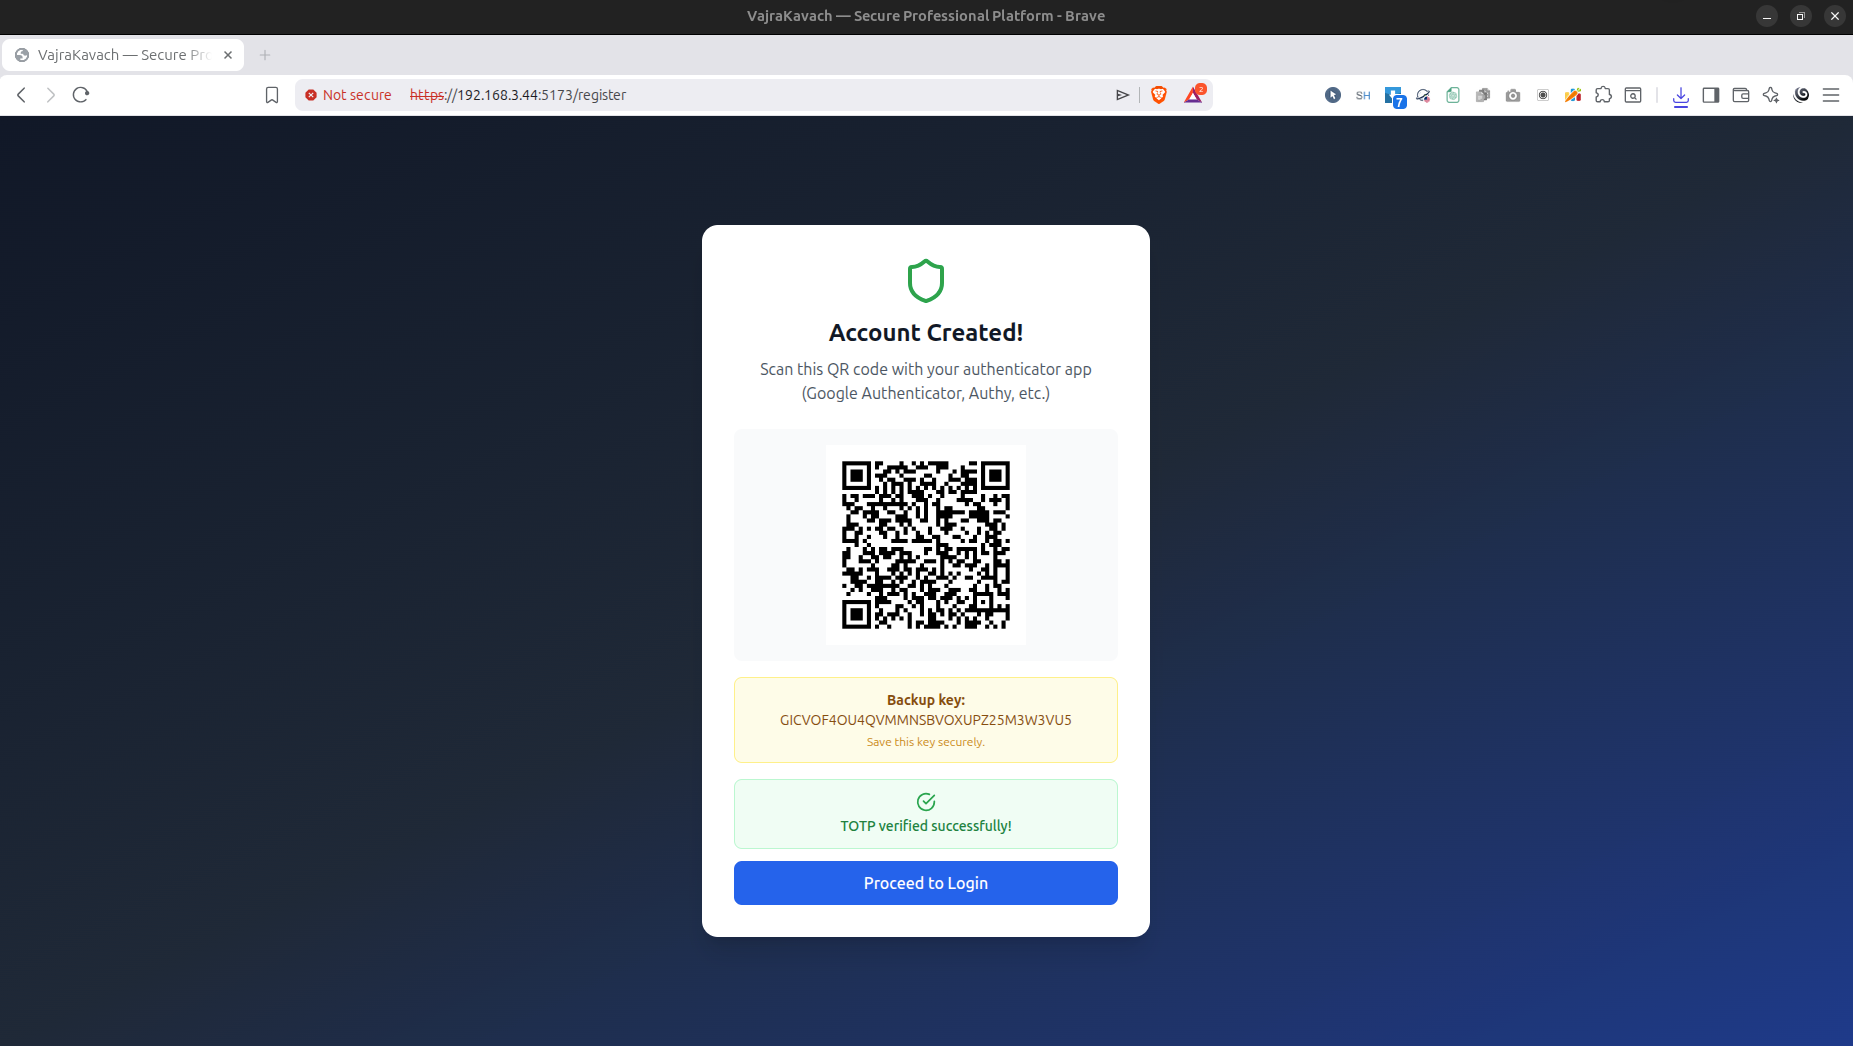
\includegraphics[width=0.7\textwidth]{screenshots/m2_totp_verify.png}
\caption{TOTP verification prompt during login}
\end{figure}

\newpage

% ============================================================
\section{User Profile Management}
% ============================================================

\subsection{Overview}
Users can create and manage rich professional profiles with field-level privacy controls.

\subsection{Profile Fields}
\begin{itemize}
  \item \textbf{Basic Info:} Full name, headline, location, bio, phone number.
  \item \textbf{Professional:} Education entries, experience entries, skills list.
  \item \textbf{Avatar:} Profile picture upload (JPEG/PNG, max 2 MB, stored as base64).
  \item \textbf{Privacy Controls:}
    \begin{itemize}
      \item Profile visibility: Public / Connections-only / Private.
      \item Show profile viewers: opt-in/opt-out toggle.
    \end{itemize}
\end{itemize}

\subsection{Profile Features}
\begin{itemize}
  \item \textbf{Profile view tracking:} Each profile visit is recorded (with 30-second deduplication cooldown). Users can see recent viewers if opted in.
  \item \textbf{Connection system:} Users can send/accept/reject/remove connection requests. The connection graph is restricted to direct connections only.
  \item \textbf{Public profiles:} Other users can visit a profile page (\texttt{/profile/:userId}) to view allowed fields.
\end{itemize}

\subsection{Screenshots}

\begin{figure}[H]
\centering
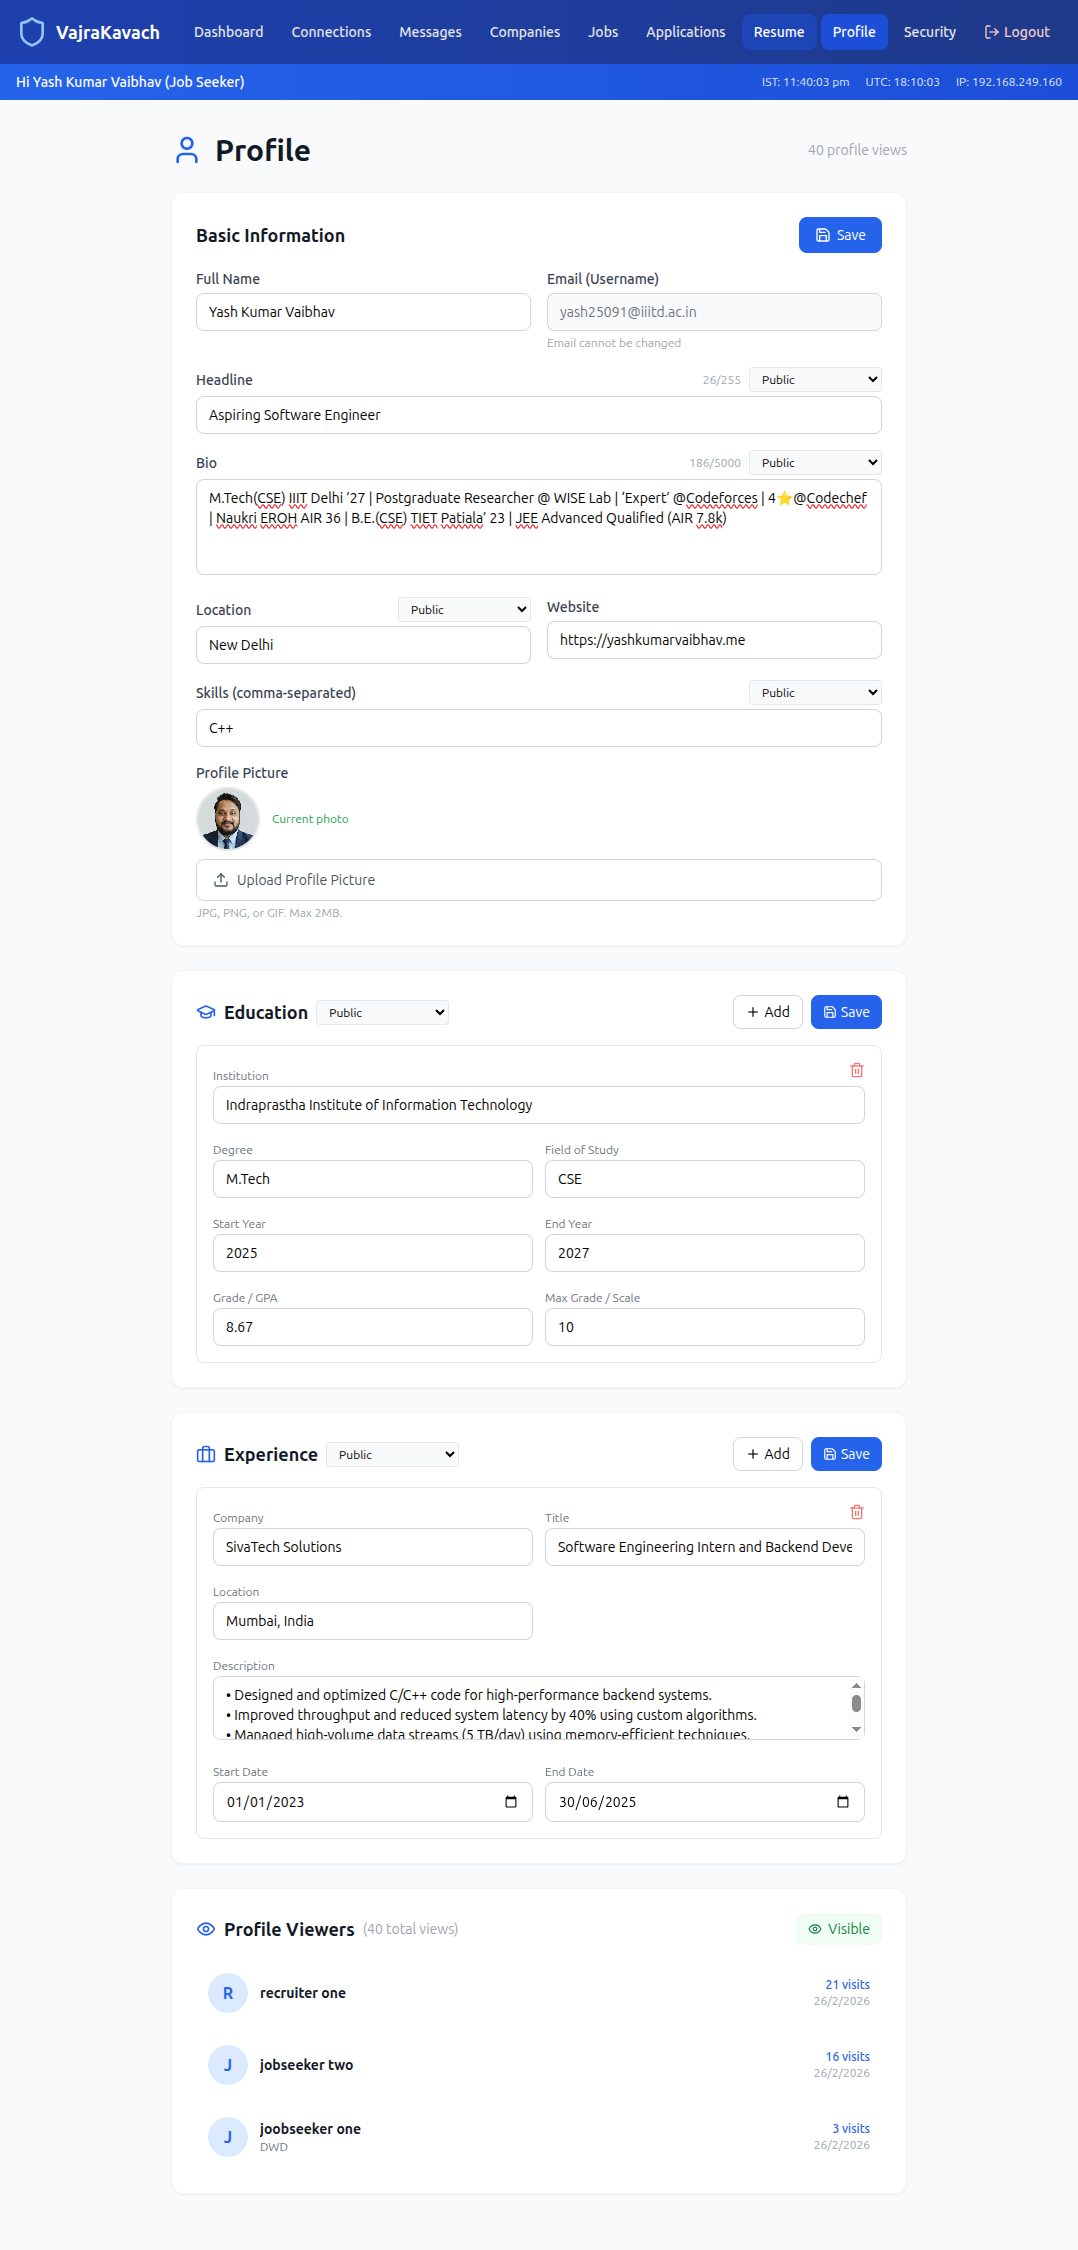
\includegraphics[width=0.85\textwidth]{screenshots/m2_profile_edit.png}
\caption{Profile edit page showing name, headline, education, experience, and skills}
\end{figure}

\begin{figure}[H]
\centering
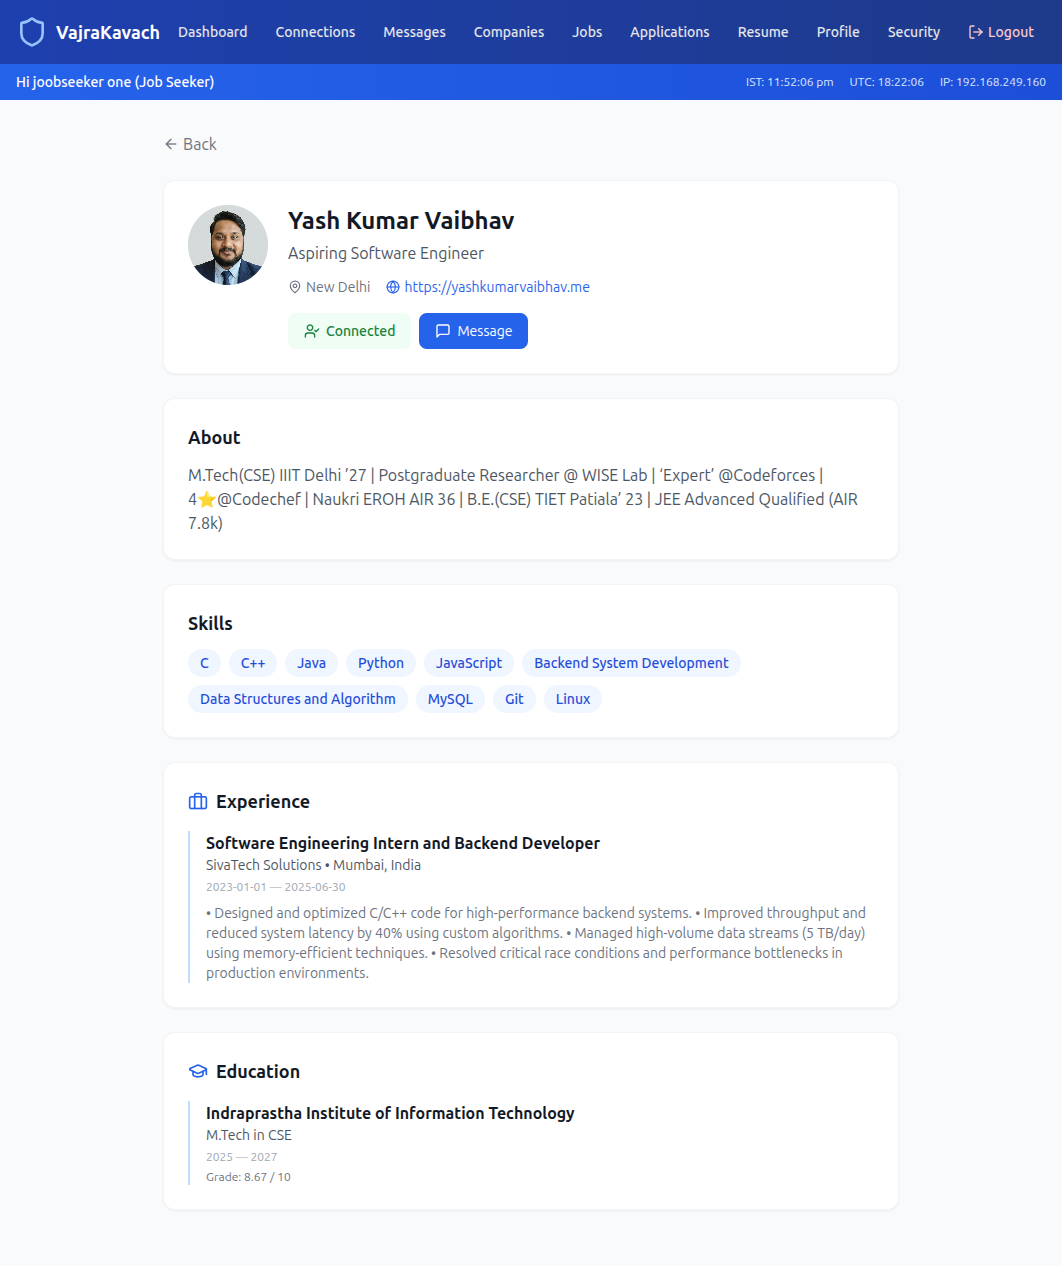
\includegraphics[width=0.85\textwidth]{screenshots/m2_profile_view.png}
\caption{Public profile view as seen by another user}
\end{figure}

\newpage

% ============================================================
\section{Secure Resume Upload with Encryption}
% ============================================================

\subsection{Overview}
Resumes are treated as sensitive assets. All uploaded resumes are encrypted at rest and subject to strict access control.

\subsection{Upload Flow}
\begin{enumerate}
  \item User uploads a PDF or DOCX file (max 10 MB).
  \item The server validates the MIME type (\texttt{application/pdf}, \texttt{application/vnd.openxmlformats...}).
  \item The file content is encrypted using \textbf{Fernet symmetric encryption} (AES-128-CBC with HMAC-SHA256 for integrity).
  \item The encrypted blob is written to disk at \texttt{backend/encrypted\_resumes/}.
  \item Metadata (original filename, MIME type, file size, encrypted path) is stored in PostgreSQL.
\end{enumerate}

\subsection{Access Control}
\begin{table}[H]
\centering
\begin{tabular}{lcc}
\toprule
\textbf{Role} & \textbf{View/Download} & \textbf{Delete} \\
\midrule
Resume Owner & Yes (TOTP for download) & Yes (TOTP required) \\
Recruiter (of applied job) & Yes (TOTP for download) & No \\
Platform Admin & Yes (TOTP for download) & Yes \\
Other Users & No & No \\
\bottomrule
\end{tabular}
\caption{Resume Access Control Matrix}
\end{table}

\subsection{Encryption Details}
\begin{itemize}
  \item \textbf{Algorithm:} Fernet (AES-128-CBC + HMAC-SHA256).
  \item \textbf{Key:} Stored in server environment configuration (never in source code).
  \item \textbf{At rest:} Only ciphertext is stored on disk. Decryption happens on-the-fly at download time.
  \item \textbf{TOTP gate:} Every download request requires a valid TOTP code, preventing unauthorized bulk access even with a valid session.
\end{itemize}

\subsection{Screenshots}

\begin{figure}[H]
\centering
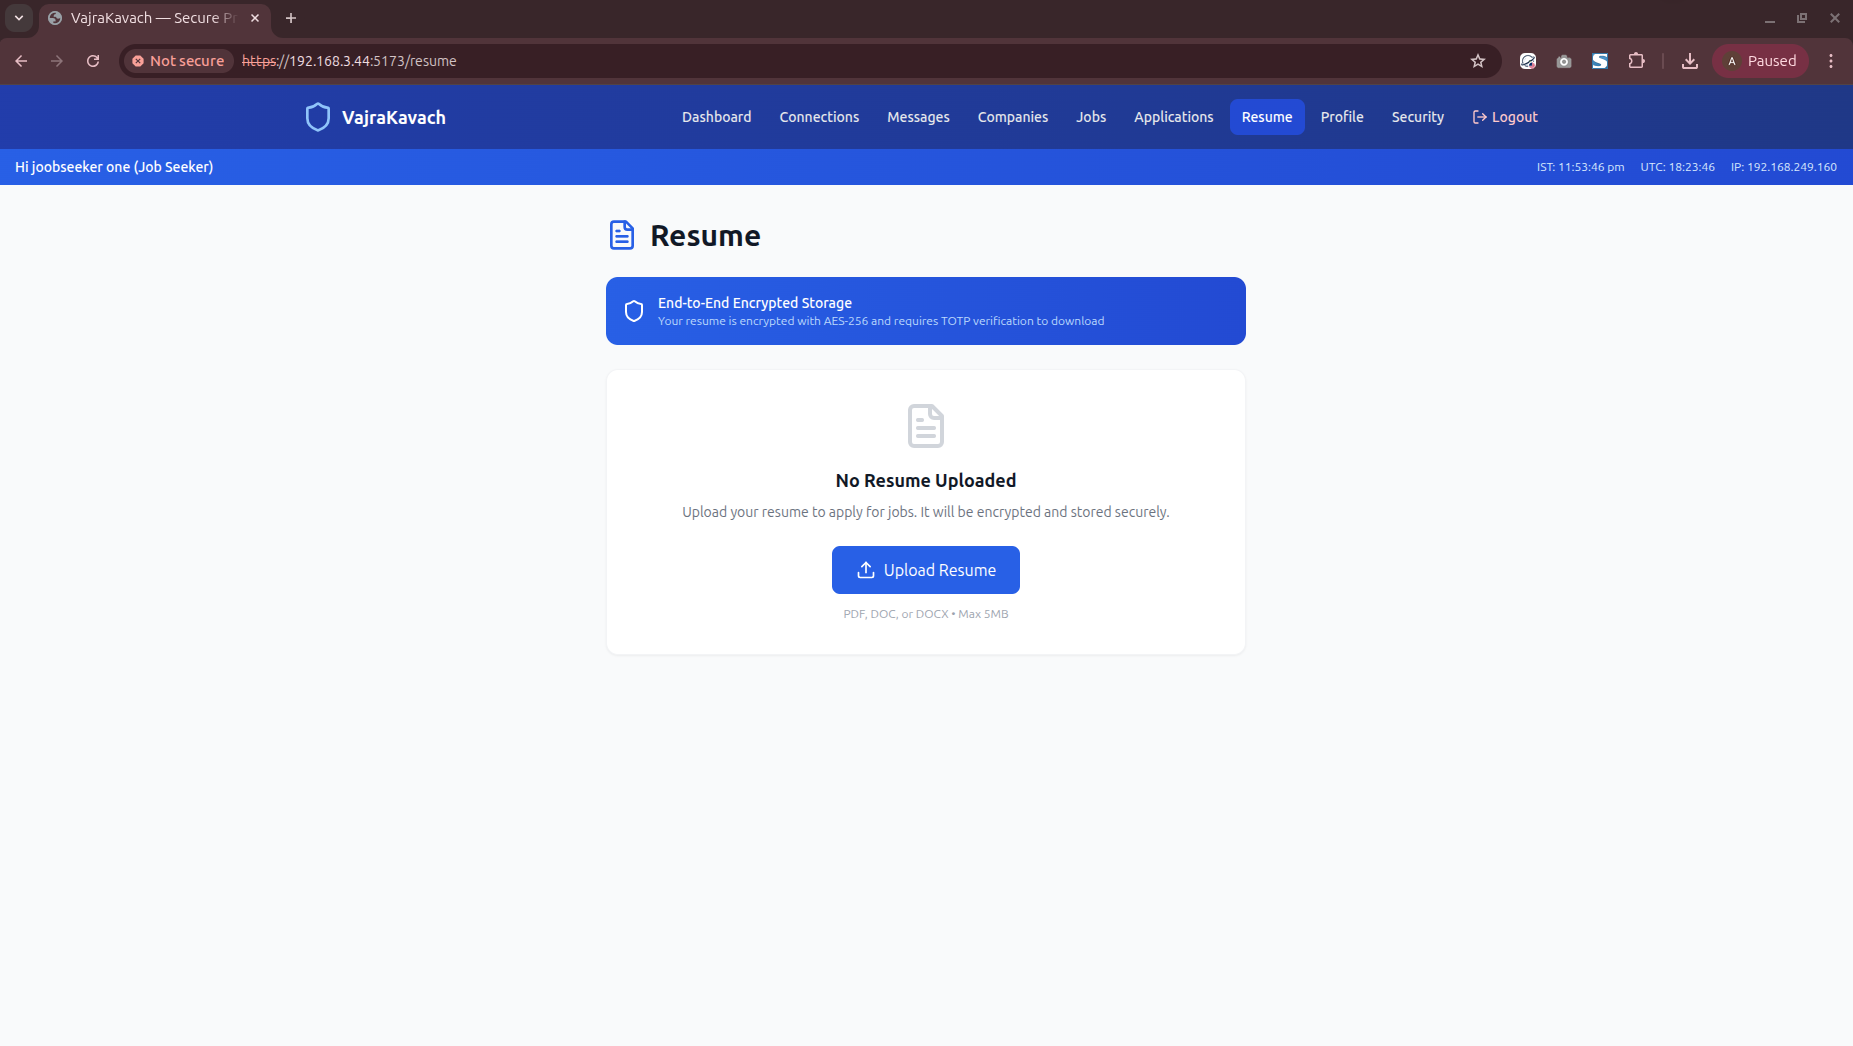
\includegraphics[width=0.85\textwidth]{screenshots/m2_resume_upload.png}
\caption{Resume upload interface showing file selection and upload button}
\end{figure}

\begin{figure}[H]
\centering
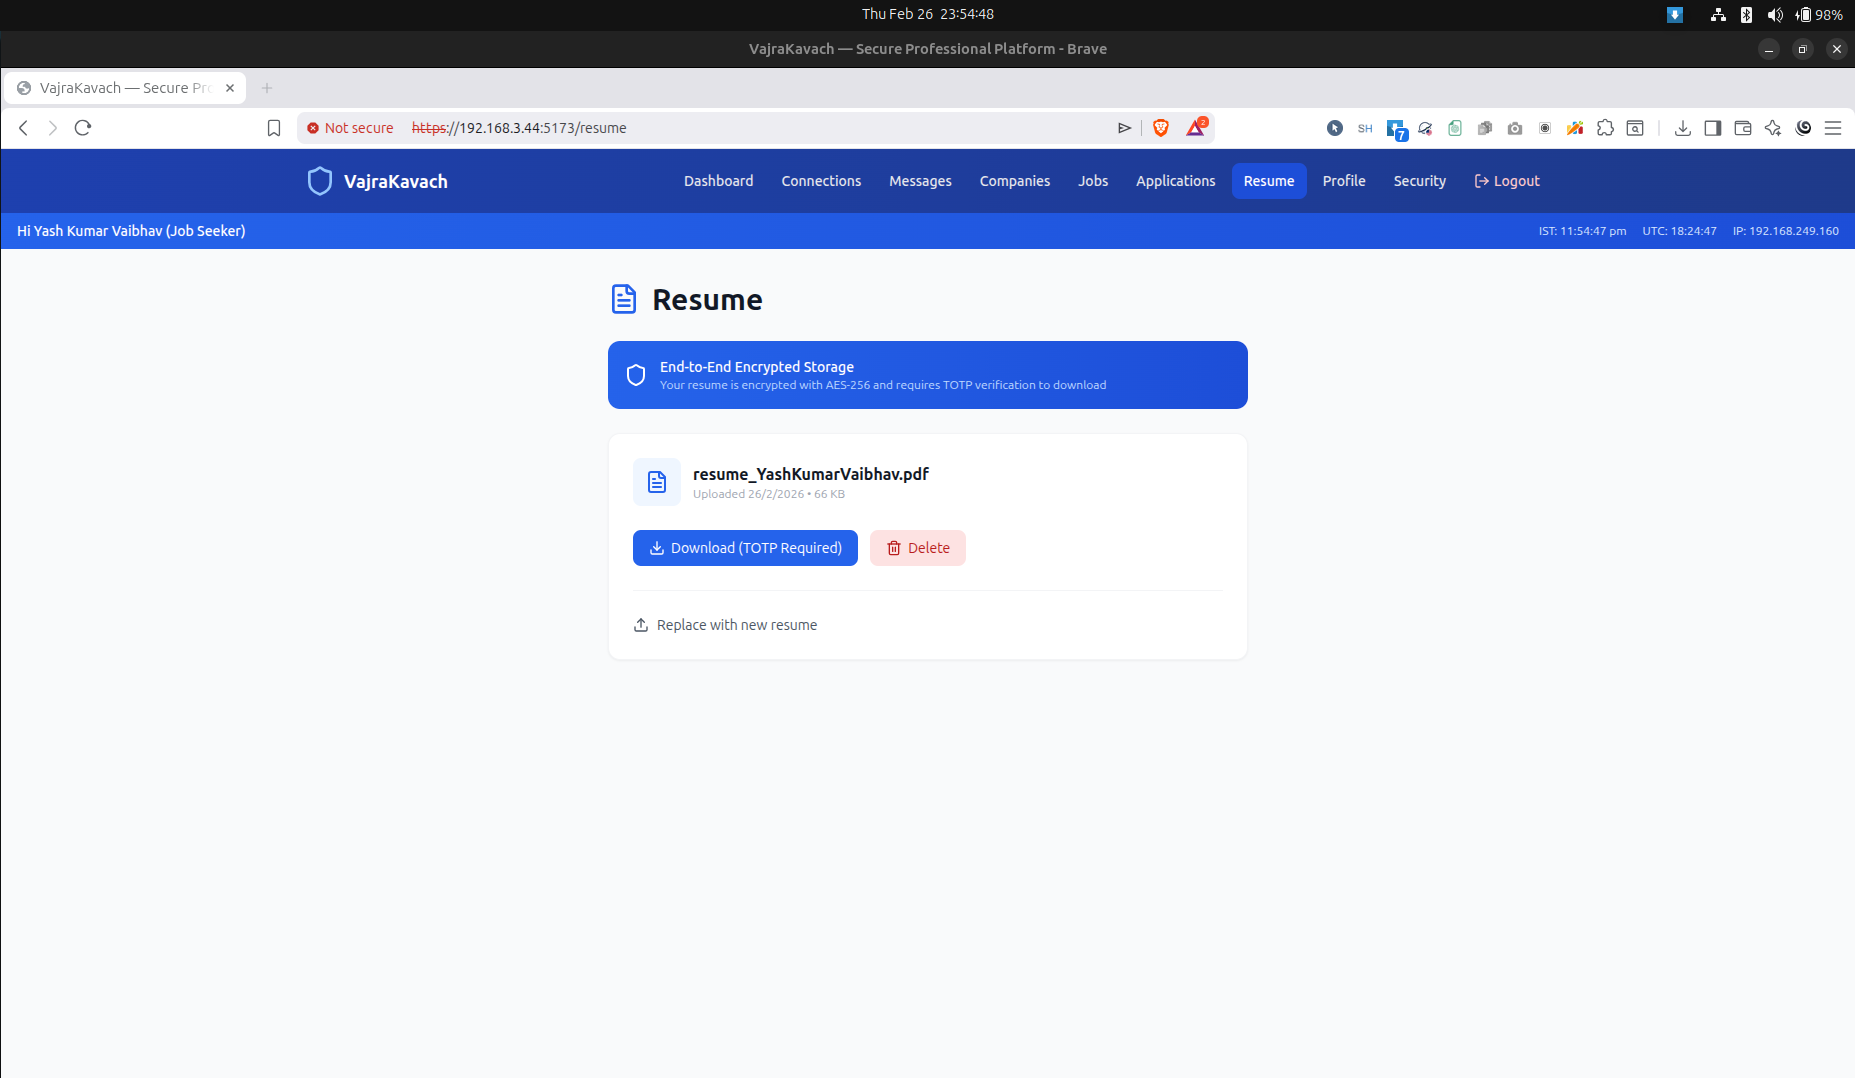
\includegraphics[width=0.85\textwidth]{screenshots/m2_resume_list.png}
\caption{User's uploaded resumes with download (TOTP-gated) and delete options}
\end{figure}

\newpage

% ============================================================
\section{Basic Admin Dashboard}
% ============================================================

\subsection{Overview}
The platform includes a dedicated admin dashboard accessible only to users with the \texttt{admin} role. It provides centralized management of users, jobs, resumes, announcements, reports, and audit logs.

\subsection{Admin Capabilities}

\begin{itemize}
  \item \textbf{Overview Tab:} Summary statistics --- total users, active users, jobs, applications, resumes, messages.
  \item \textbf{User Management:}
    \begin{itemize}
      \item View all registered users with search and role filtering.
      \item Suspend or reactivate user accounts.
      \item Delete user accounts.
      \item Role-based access control (RBAC): Regular User, Recruiter, Admin.
    \end{itemize}
  \item \textbf{Job Management:} View and delist job listings.
  \item \textbf{Resume Management:} View all uploaded resumes with download capability (TOTP-gated).
  \item \textbf{Announcements:} Post encrypted announcements visible to all users.
  \item \textbf{Reports:} Review user reports (spam, harassment, fraud, etc.) and take action (review, resolve, dismiss).
  \item \textbf{Audit Logs:} View tamper-evident logs of all critical actions with hash chaining.
\end{itemize}

\subsection{Role-Based Access Control (RBAC)}
\begin{table}[H]
\centering
\begin{tabular}{lccc}
\toprule
\textbf{Action} & \textbf{Job Seeker} & \textbf{Recruiter} & \textbf{Admin} \\
\midrule
View own profile & \checkmark & \checkmark & \checkmark \\
Apply to jobs & \checkmark & & \\
Post jobs & & \checkmark & \\
Manage users & & & \checkmark \\
View audit logs & & & \checkmark \\
Suspend accounts & & & \checkmark \\
\bottomrule
\end{tabular}
\caption{RBAC Permission Matrix}
\end{table}

\subsection{Screenshots}

\begin{figure}[H]
\centering
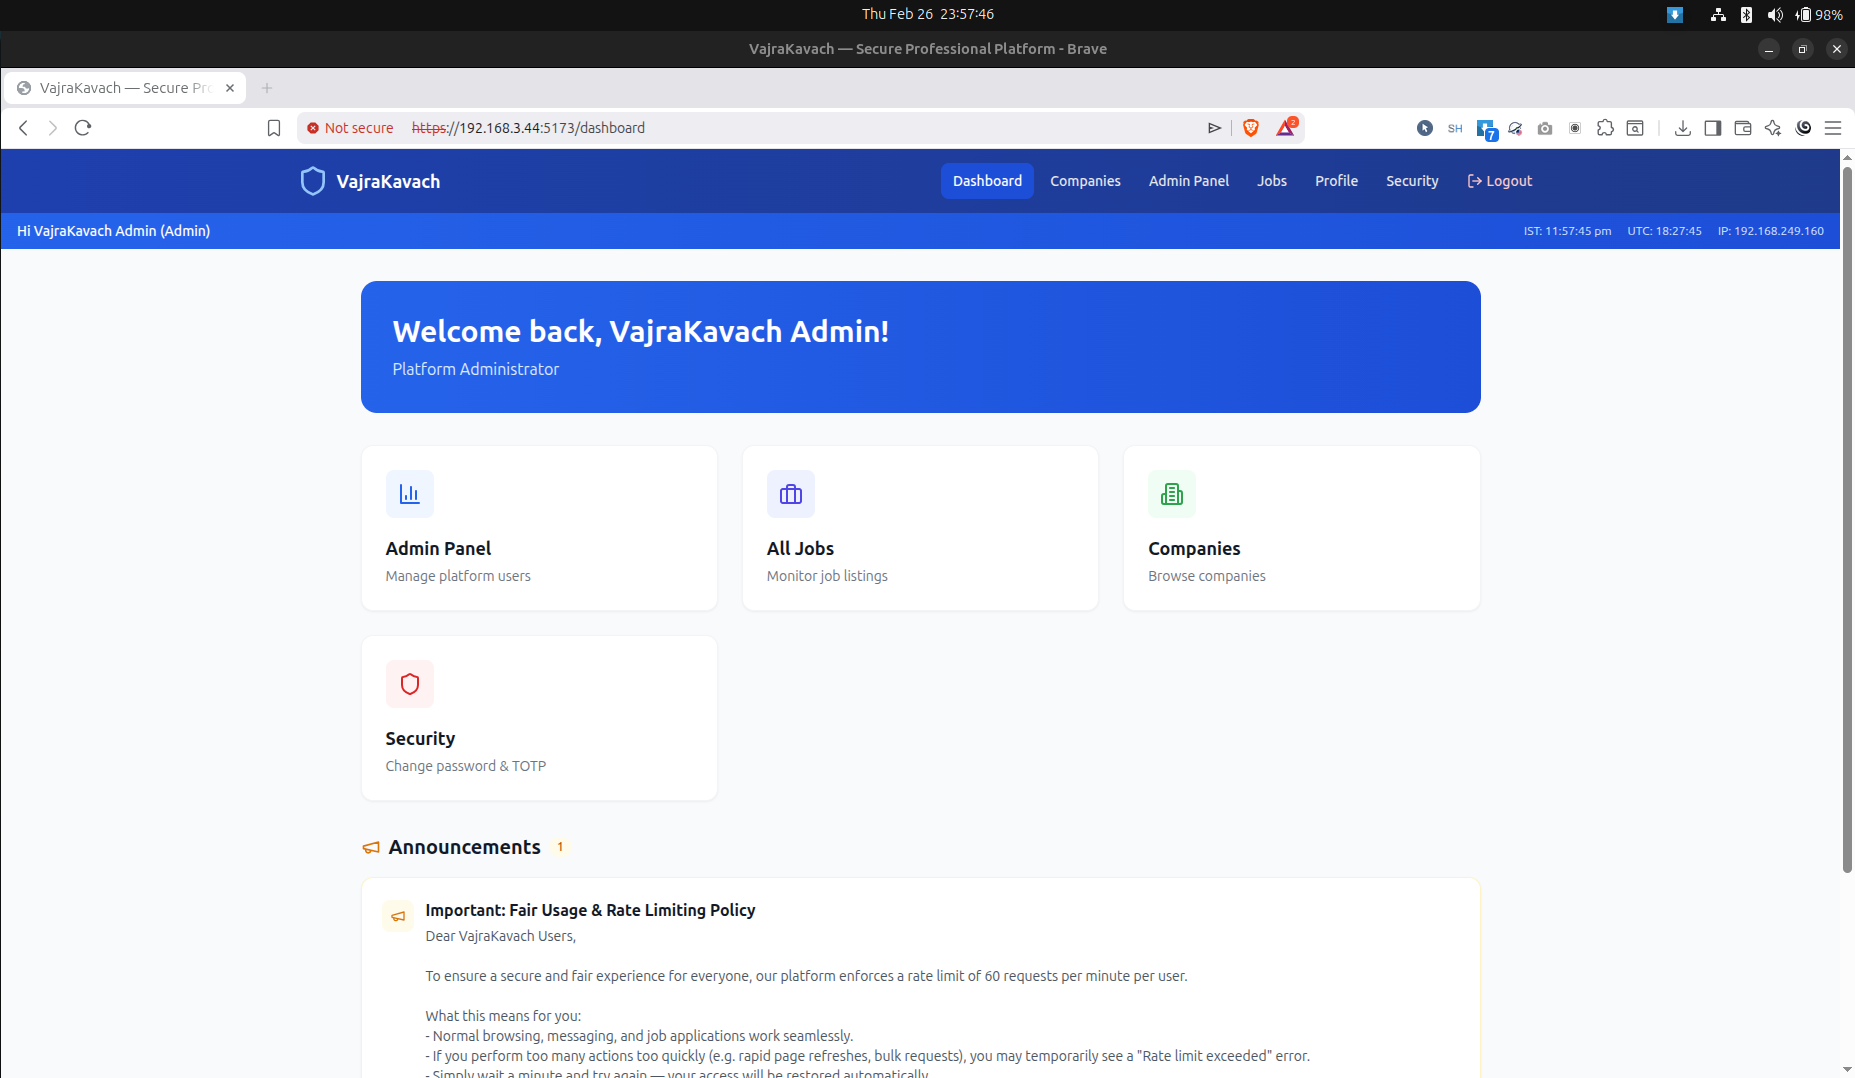
\includegraphics[width=0.85\textwidth]{screenshots/m2_admin_overview.png}
\caption{Admin dashboard overview showing platform statistics}
\end{figure}

\begin{figure}[H]
\centering
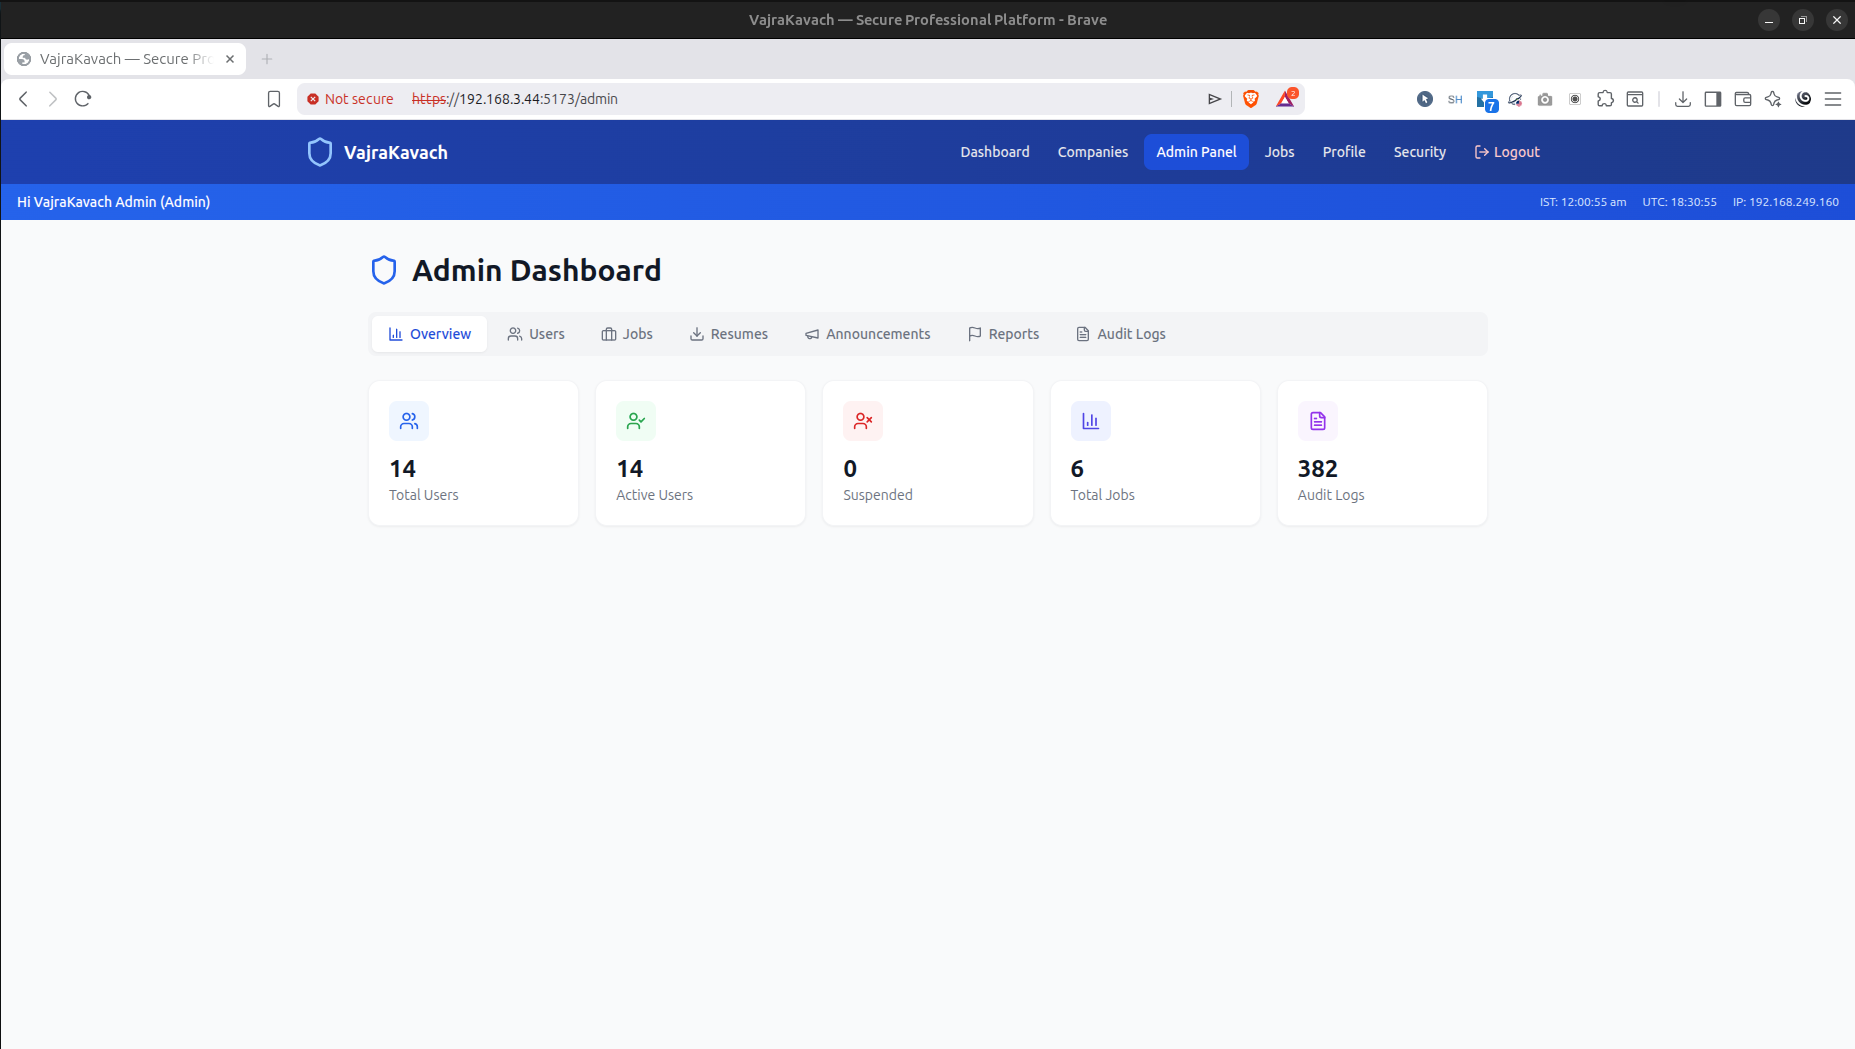
\includegraphics[width=0.85\textwidth]{screenshots/m2_admin_users.png}
\caption{Admin user management panel with search, suspend, and delete controls}
\end{figure}

\newpage

% ============================================================
\section{Summary}
% ============================================================

Milestone~2 delivers the core authentication and user management features of VajraKavach:

\begin{enumerate}
  \item \textbf{Secure Registration \& Login} --- Argon2id password hashing, JWT tokens with IP binding, Pydantic input validation.
  \item \textbf{TOTP Two-Factor Authentication} --- Mandatory TOTP setup and verification on login, plus TOTP gates on high-risk actions (resume download/delete, password change).
  \item \textbf{User Profile Management} --- Rich profiles with education, experience, skills, avatar upload, field-level privacy controls, and profile view tracking.
  \item \textbf{Encrypted Resume Storage} --- Fernet AES encryption at rest, strict RBAC access control, TOTP-gated downloads.
  \item \textbf{Admin Dashboard} --- Centralized management of users, jobs, resumes, announcements, reports, and audit logs with role-based access control.
\end{enumerate}

\vspace{0.5cm}
\noindent All security measures follow best practices as outlined in the course requirements. The codebase is version-controlled and ready for Milestone~3 (company pages, job workflows, messaging, and initial audit logging).

\vspace{1cm}
\noindent\textbf{Repository:} \url{https://github.com/yashkumarvaibhav/VajraKavach}

\end{document}
